%LaTeX SAMPLE FILE FOR PAPERS OF CDAM

% LaTeX 2e
\documentclass[12pt]{article}

\usepackage{graphicx}
\usepackage{epsfig}
\usepackage{cite}
\usepackage{amsmath,amssymb,amsfonts,amsthm}
\usepackage[boxed]{algorithm2e}
\usepackage{caption}
\usepackage{wrapfig}
\usepackage{upgreek}
\usepackage{adjustbox}
\usepackage{pbox}
\usepackage{index}
\usepackage{color}
\usepackage{makecell}
\usepackage{multirow}
\usepackage{bbm}
\usepackage{lastpage}
\usepackage{longtable}
\usepackage{changepage}

% LaTeX 2.09
%\documentstyle[12pt]{article}

%%%%%%%%%%%%%%%%%%%%%%%%%%%% paper layout %%%%%%%%%%%%%%%%%%%%%%%%%%%%%%
\hoffset=-1in
\voffset=-1in
% Please, don't change this layout
\parindent=6mm
\topskip=0mm
\topmargin=30mm
\oddsidemargin=27.5mm
\evensidemargin=27.5mm
\textwidth=155mm
\textheight=237mm
\headheight=0pt
\headsep=0pt
\footskip=2\baselineskip
\addtolength{\textheight}{-\footskip}

\providecommand{\keywords}[1]
{
\vspace{2mm}\hspace{20pt}\textbf{\textit{Keywords:}} #1
}

\providecommand{\abskeyw}[2]
{
\begin{small}
\begin{adjustwidth}{10mm}{10mm}
\vspace{1mm}\hspace{20pt}#1

\keywords{#2}
\end{adjustwidth}
\end{small}
}

% To remove after translation
\usepackage[T2A]{fontenc}
\usepackage[utf8]{inputenc}
\usepackage[english,russian]{babel}
\usepackage{bm}

\begin{document}

%%% Title section
\begin{center}
{\Large\bf Monte Carlo SSA for extracting weak signals}\\\vspace{2mm} {\sc E. Poteshkin$^1$, N. Golyandina$^2$}\\\vspace{2mm}
{\it $^{1}$ $^{2}$St.Petersburg State University\\
%$^{2}$Institute  ...\\
St.Petersburg, Russia\\} e-mail: {\tt $^1$ivanov@yandex.ru,
$^2$n.golyandina@spbu.ru}

\abskeyw{В работе рассматривается задача выделения сигнала из шума методом анализа сингулярного спектра (SSA). Предлагается алгоритм автоматического выделения значимых модулированных гармоник без задания их периодов, который на основе критерия Monte Carlo SSA определяет значимые частоты и затем выделяет их.}{time series, signal extraction, signal detection, singular spectrum analysis}
\end{center}

\section{Введение}

Рассмотрим следующую модель: $\mathsf{X}=\mathsf{S}+\mathsf{R}$, где $\mathsf{X} = (x_1,\ldots,x_N)$~--- наблюдаемый временной ряд, $\mathsf{S}$~--- сигнал, $\mathsf{R}$~--- шум, т.е. реализация некоторого стационарного процесса. В работе рассматриваются две проблемы: проблема обнаружения сигнала $\mathsf{S}$ и проблема выделения сигнала при его наличии.

Для решения первой проблемы используется метод Monte Carlo SSA (MC-SSA)~\cite{AllenSmith96}, проверяющий гипотезу $H_0:\mathsf{S}=0$, а для решения второй~--- метод анализа сингулярного спектра (singular spectrum analysis, SSA)~\cite{Broomhead1986, ssa2001}, раскладывающий ряд на элементарные компоненты, после группировки которых получается разложение ряда на тренд, периодические компоненты и шум. Один из шагов SSA подразумевает визуальный анализ для определения компонент сигнала, поэтому возникает потребность в автоматизации этого шага, этой проблеме посвящены, например, работы~\cite{alexandrov, Kalantari2019, circSSA, autoSSA}, посвященные, главным образом, выделению тренда или сглаживанию. Целью работы является определение подхода к автоматическому выделению слабых осциллирующих сигналов, обнаруживаемых критерием MC-SSA.

% \section{Метод SSA}

% Пусть $\mathsf{X}=(x_1,\ldots,x_N)$, $x_i\in \mathbb{R}$,~--- временной ряд длины $N$. Зафиксируем параметр $L$, $1<L<N$, называемый длиной окна и построим так называемую траекторную матрицу $\mathbf{X}=[X_1:\ldots:X_K]$, состоящую из $K=N-L+1$ векторов вложения $X_i=(x_i,\ldots,x_{i+L-1})^{\mathrm{T}}\in \mathbb R^L$.

% Следующий шаг~--- разложение в сумму матриц единичного ранга $\mathbf{X}=\sum_{i=1}^d \mathbf{X}_i$. В базовом SSA используется сингулярное разложение матрицы $\mathbf{X}$, где столбцы $\mathbf{X}_i$ состоят из проекций столбцов матрицы $\mathbf{X}$ на порождаемые ею  самой левые сингулярные векторы.

% Далее компоненты полученного матричного разложения группируются на основе свойств левых сингулярных векторов, и каждая сгруппированная матрица преобразуется во временной ряд. Таким образом, результатом SSA является разложение временного ряда.

% \section{Метод Monte Carlo SSA}

% Рассмотрим задачу поиска сигнала во временном ряде. Модель временного ряда имеет вид
% \[
%     \mathsf{X}=\mathsf{S} + \bm\xi,
% \]
% где $\mathsf{S}$~--- сигнал, $\bm\xi$~--- стационарный процесс с нулевым средним. Тогда нулевая гипотеза $H_0:\mathsf{S}=0$ и альтернатива $H_1:\mathsf{S}\ne0$.

% Зафиксируем длину окна $L$ и обозначим траекторную матрицу ряда $\boldsymbol\xi$ как $\mathbf\Xi$. Рассмотрим вектор $W\in \mathbb R^L$ единичной длины, называемый проекционным вектором. Введем величину
% \[
%     p=\left\|\mathbf\Xi^{\mathrm{T}} W\right\|^2.
% \]
% Статистикой критерия является величина
% \[
%     \widehat p = \left\|{\mathbf{X}}^{\mathrm{T}} W\right\|^2.
% \]
% Распределение статистики критерия оценивается с помощью моделирования согласно нулевой гипотезе, отсюда и название метода.

% Если вектор $W$~--- синусоида с частотой $\omega$, то $\widehat{p}$ отражает вклад частоты $\omega$ в исходный ряд. Так как частота ожидаемого сигнала неизвестна, то необходимо рассматривать несколько векторов $W_k$, $k=1,\ldots,H$. Решение возникающей при этом проблемы множественного тестирования рассматривается в~\cite{Golyandina2023}.
% Гипотеза об отсутствии сигнала отвергается, если хотя бы для одного вектора $W=W_k$ значение $\widehat p$ оказывается значимым.

% Важной частью метода MC-SSA является способ выбора векторов $W_k$. В данной работе в качестве векторов для проекции берутся косинусы с равноотстоящими частотами $\omega_k=k/(2L)$, $k=1,\ldots,L$. В этом случае можно говорить о значимых частотах, присутствующих в сигнале.

\section{Метод autoMCSSA}
Для описания разработанного метода необходимо ввести некоторые обозначения и предположения.

В предлагаемом алгоритме используется модификация MC-SSA с поправкой на множественные сравнения~\cite{Golyandina2023}. В качестве векторов для проекции, необходимых для построения статистики критерия, были выбраны косинусы с равноотстоящими частотами $\omega_k=k/(2L)$, $k=1,\ldots,L$. В этом случае можно говорить о значимых частотах, присутствующих в сигнале.

Для ряда $\mathsf{X}$ длины $N$ и $0\leqslant\omega_1\leqslant\omega_2\leqslant0.5$ будем использовать ту же меру, что в~\cite{alexandrov} для выделения тренда.
Пусть мера $T(\mathsf{X};\omega_1,\omega_2)$ отражает долю вклада частот из интервала $[\omega_1,\omega_2)$, сосчитанную на основе значения периодограммы ряда. 

\begin{figure}[htbp]
    \centering
    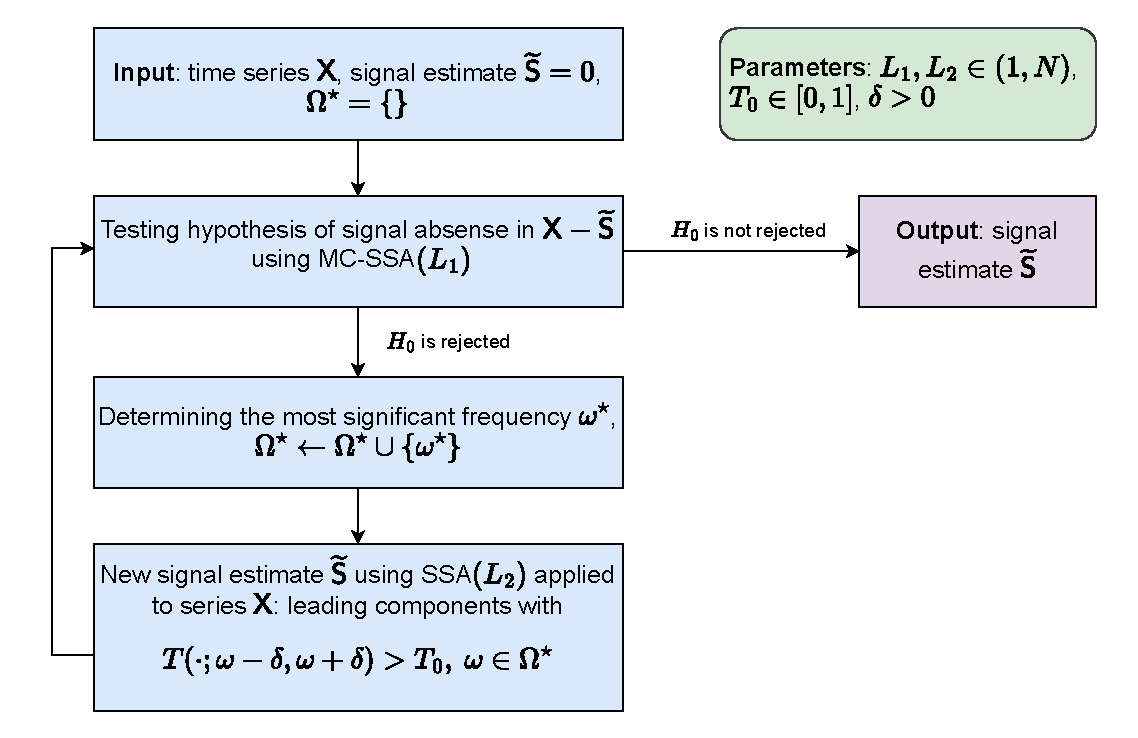
\includegraphics[width=\textwidth]{img/auto_mcssa_alg.pdf}
    \caption{Алгоритм autoMCSSA}
    \label{fig:autoMCSSA_alg}
\end{figure}

На рис.~\ref{fig:autoMCSSA_alg} изображена блок-схема алгоритма autoMCSSA. Заключается он в последовательном применении критерия MC-SSA до тех пор, пока гипотеза не перестанет отвергаться. Если на очередной итерации алгоритма гипотеза отвергается, определяется максимально значимая частота $\omega^\star$ и вычисляется новая оценка сигнала с помощью SSA,примененного к исходному ряду: для каждой частоты $\omega$ из множества значимых частот $\Omega^\star$ выбираются первые компоненты с мерой $T$ превышающей порог $T_0$. Как только гипотеза перестает отвергаться, алгоритм завершает свою работу и тогда $\widetilde{\mathsf{S}}$~--- итоговая оценка сигнала.

Оценивать частоту $\omega^\star$ будем с помощью взвешенной суммы ближайщих значимых частот с весами, определяемыми их значимостью. 
Такой способ оценки позволяет получить более точную оценку $\omega$ в случае, когда она не попадает в решетку $k/(2L)$.

Рассмотрим пример работы рассмотренного алгоритма. Пусть $\mathsf{X}=\mathsf{S}+\bm{\xi}$, где $\bm\xi$~--- модель AR(1) с параметрами $\phi=0.7$ и $\sigma^2=1$, $N=200$, $\mathsf{S}=(s_1,\ldots, s_N)$,
\[
s_n=0.075\, e^{0.02n}\cos(2\pi n/8) + 2\cos(2\pi n / 4) + 0.2\cdot(-1)^n.
\]


\begin{figure}[!h]
    \centering
    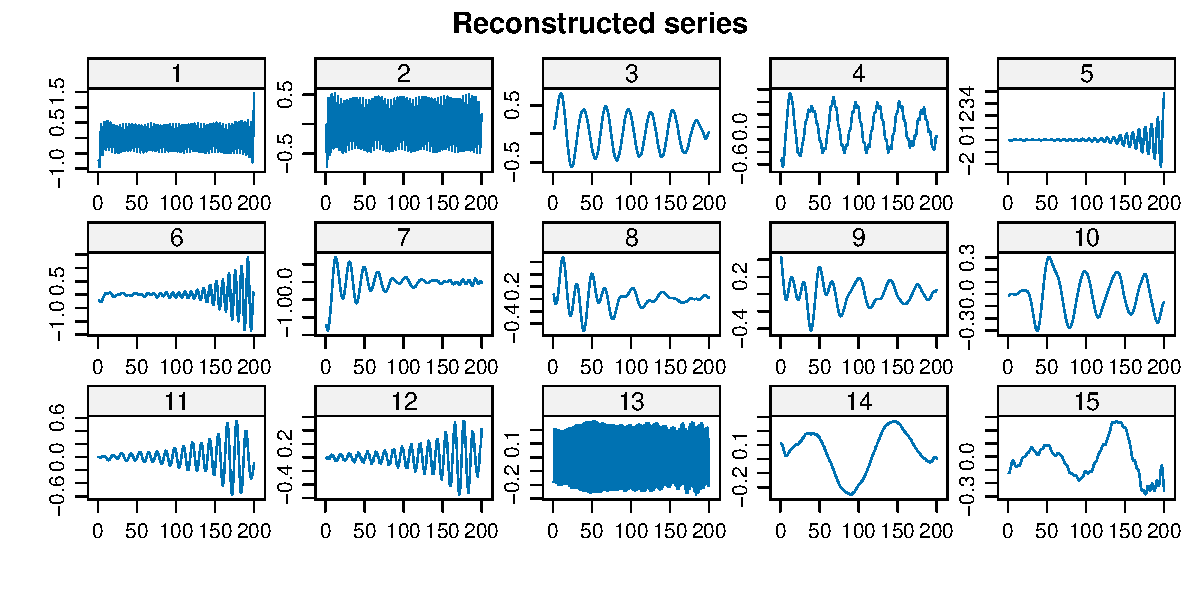
\includegraphics[width=0.8\textwidth]{img/reconstructed_ts.pdf}
    \caption{Элементарные восстановленные компоненты}
    \label{fig:reconstructed_ts}
\end{figure}

\begin{figure}[!h]
    \centering
    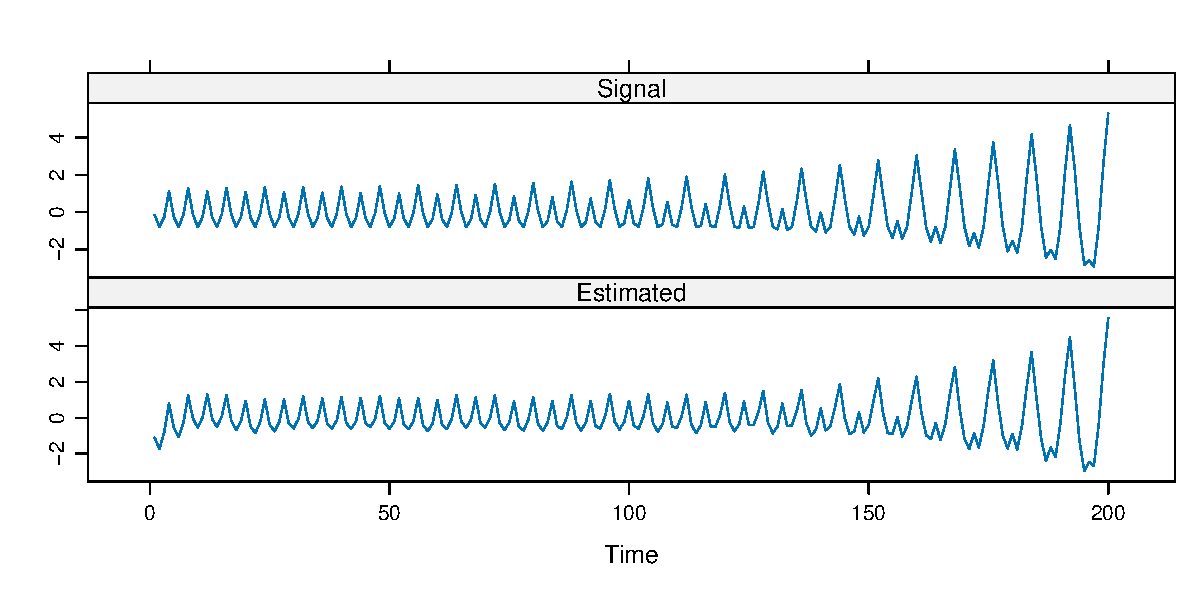
\includegraphics[width=0.8\textwidth]{img/auto_mcssa_result.pdf}
    \caption{Результат autoMCSSA ($L_1=50$, $L_2=100$, $\delta=1/80$, $T_0=0.5$)}
    \label{fig:autoMCSSA_res}
\end{figure}

На рис.~\ref{fig:reconstructed_ts} представлены первые $15$ элементарных восстановленных с помощью SSA компонент. Сигналу соответствуют компоненты с индексами $1$, $2$, $5$, $6$ и $13$. Не видя формулы, по которой этот сигнал задается, сказать наверняка, какие компоненты неслучайные, проблематично, поскольку компоненты $3$, $4$ и $11$, $12$ похожи на пары гармоник. Мы применили алгоритм autoMCSSA к этому ряду и получили, что разработанный метод правильно идентифицировал компоненты, соответствующие сигналу, на рис.~\ref{fig:autoMCSSA_res} представлены истинная форма сигнала $\mathsf{S}$ и его оценка методом autoMCSSA.

\section{Заключение}
Таким образом, в работе предлагается алгоритм, способный выделить только значимые компоненты, при этом не требуется задавать период для периодической компоненты, периодик может быть несколько с неизмеримыми периодами и они могут быть модулированными с разной амплитудной модуляцией. 

%% please make bibitems content in a style below !!!
%% papers with "free style" bibitems content will be rejected !!!

\begin{thebibliography}{10}

    \bibitem{AllenSmith96} Allen~M., Smith~L. Monte Carlo SSA: detecting irregular oscillations in the presence of coloured noise // Journal of Climate.~--- 1996.~--- Vol.~9.~--- P.~3373--3404.
    \bibitem{Broomhead1986} Broomhead~D., King~G. Extracting qualitative dynamics from experimental data // Physica D: Nonlinear Phenomena.~--- 1986.~--- Vol. 20, no. 2–3.~--- P.~217--236.
    \bibitem{ssa2001} Golyandina~N., Nekrutkin~V., Zhigljavsky~A. Analysis of Time Series Structure: SSA and Related Techniques.~--- Chapman and Hall/CRC, 2001.
    \bibitem{alexandrov} Alexandrov Th. A method of trend extraction using singular spectrum analysis // RevStat.~--- 2009~--- Vol.~7 no~1.~--- P.~1-–22.
    .~--- 2004.~--- Vol.~7-80.~--- P.~54--61.
    \bibitem{Kalantari2019} Kalantari~M., Hassani.~H. Automatic grouping in singular spectrum analysis // Forecasting.~--- 2019.~--- Vol. 1, no 1.~--- P.~189--204.
    \bibitem{circSSA} Bogalo~J., Poncela~P., Senra~E. Circulant singular spectrum analysis: A new automated procedure for signal extraction // Signal Processing.~--- 2021.~--- Vol.~179.
    \bibitem{autoSSA} Golyandina~N., Dudnik~P., Shlemov~A. Intelligent Identification of Trend Components in Singular Spectrum Analysis // Algorithms.~--- 2023.~--- Vol. 16.~--- ID 353.
    \bibitem{Golyandina2023} Golyandina~N. Detection of signals by Monte Carlo singular spectrum analysis: multiple testing // Statistics and Its Interface.~--- 2023.~--- Vol.~16. no~1.~--- P.~147--157.

\end{thebibliography}


\end{document}
